\documentclass[12pt,titlepage,oneside]{memoir}
\usepackage{graphicx}
\usepackage{amsmath}
\usepackage{amsfonts}
\usepackage{amssymb}
\usepackage{hyperref}


\chapterstyle{southhall}
\newcommand{\HRule}{\rule{\linewidth}{0.5mm}}
\pagestyle{plain}
\setstocksize{11in}{8.5in}
\settrimmedsize{11in}{8.5in}{*}
\settrims{0in}{0in}
\settypeblocksize{8.5in}{35pc}{*}
\setlrmargins{1in}{*}{*}
\setulmargins{1in}{*}{*}
\setheadfoot{13pt}{26pt}
\setheaderspaces{*}{13pt}{*}
\checkandfixthelayout


\begin{document}
\begin{titlingpage}
\begin{center}


\vspace{50mm}
% Title
\HRule \\[0.4cm]
{ \huge \bfseries Raspberry Robot Build Instructions}\\[0.4cm]

\HRule \\[1.5cm]

% Author and supervisor
\begin{minipage}{0.4\textwidth}
\begin{flushleft} \large
\emph{Author:}\\
Robbie \textsc{Edwards}\\
\end{flushleft}
\end{minipage}
\vfill
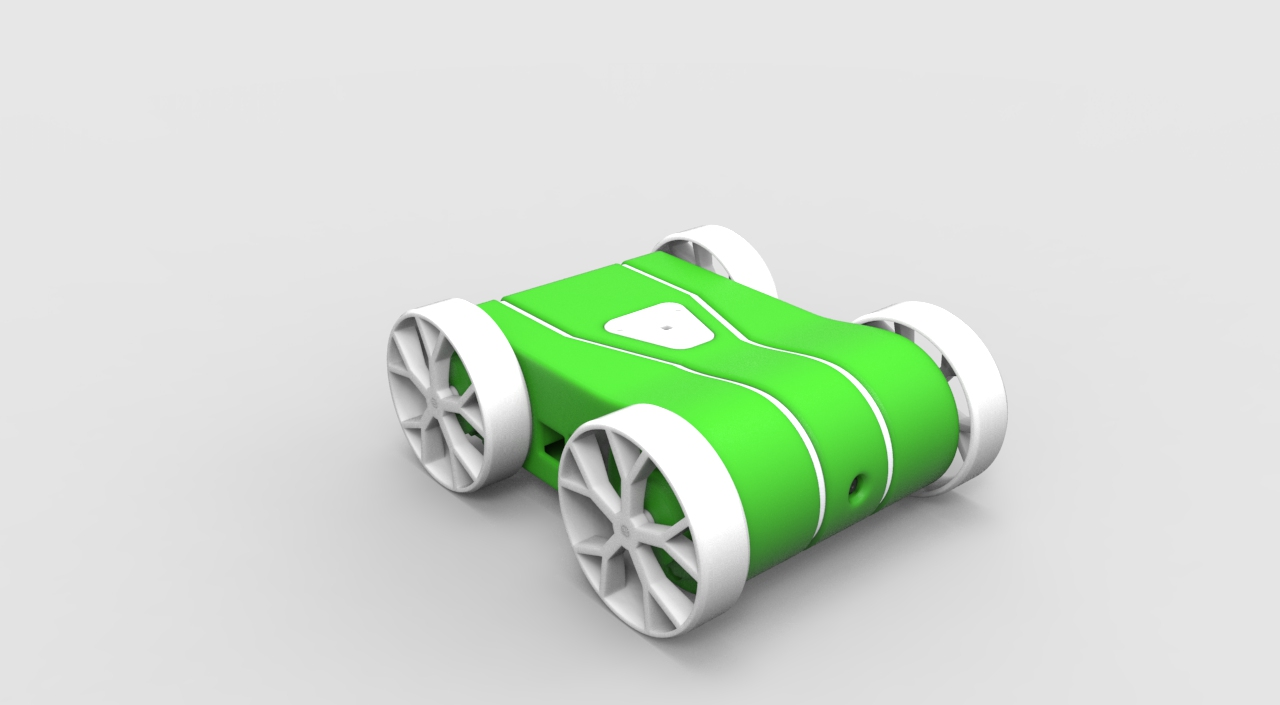
\includegraphics[width=450px]{render/pibot2.jpg}
\vspace*{1cm}

% Bottom of the page
{\large \today}

\end{center}
\end{titlingpage}


%\frontmatter
%\tableofcontents

\mainmatter
\counterwithout{figure}{chapter}
%\section{Introduction}
%This document presents a brief overview of some of the many personal and academic projects carried out by Robbie Edwards. Further documentation is available upon request for the listed projects or on any of the work related or artistic projects not shown here. 

\chapter{Overview}
%\begin{figure}[!ht]
%\includegraphics[width=500px]{pawly.pdf}
%\centering
%\end{figure}

The Raspberry Robot was created to provide a low cost Linux/Robot Operating System (ROS) enabled mobile robot platform. It currently runs ROS Indigo and Raspbian Jessie. The \href{http://wiki.ros.org/ROS/Introduction}{Robot Operating System} is a BSD licensed meta-operating system which provides a convenient set of tools for developing software for robot applications. It is well documented online and explained in further detail in various \href{http://wiki.ros.org/Books}{books}. Many open source ROS packages are freely available to carry out robot related software tasks ranging from interfacing with sensor hardware to carrying out navigation and mapping \\



\section{Features}:
\begin{itemize}
\item Raspberry Pi with Raspbian Jessie
\item ROS Indigo
\item Independent Motor Control of each wheel
\item WS2812b Status LED
\item Raspberry Pi camera
\item Lithium Battery: Turnigy Nanotech 3S 2200mAh,
\item 2 hour or greater run time
\item USB ports
\item Wifi expandable
\item Logitech F710 Game pad expandable
\end{itemize}

\pagebreak
\begin{figure}[!htbp]
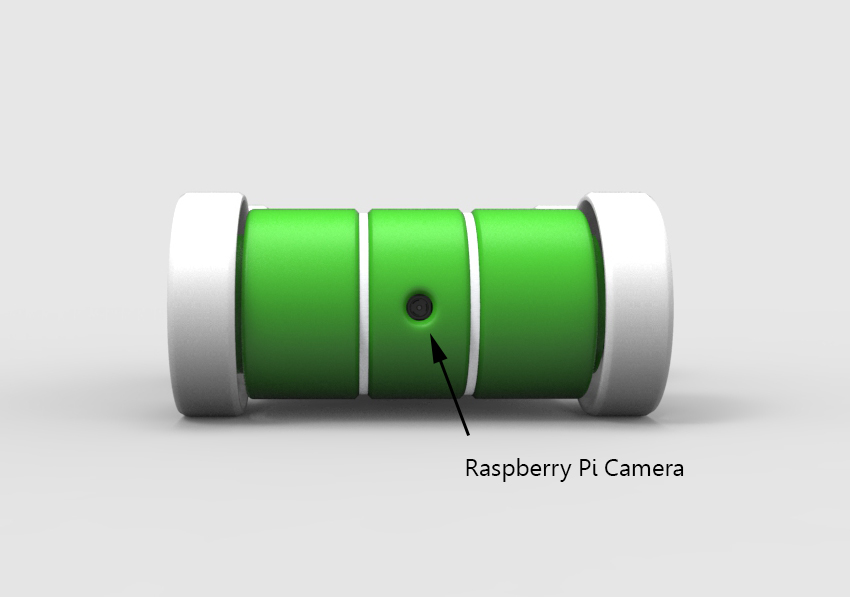
\includegraphics[width=350px]{render/pibotfront.jpg}
\centering
\end{figure}

\begin{figure}[!htbp]
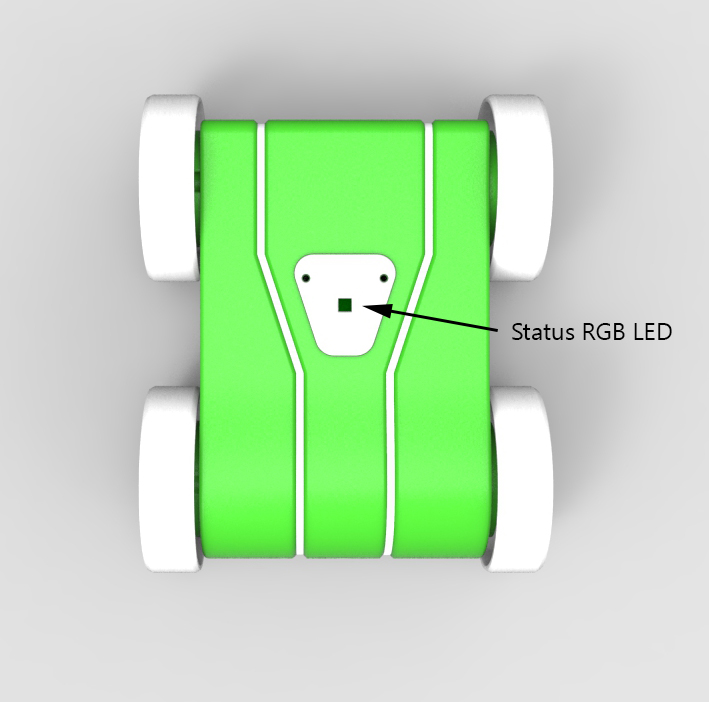
\includegraphics[width=350px]{render/pibottop.jpg}
\centering
\end{figure}

\begin{figure}[!htbp]
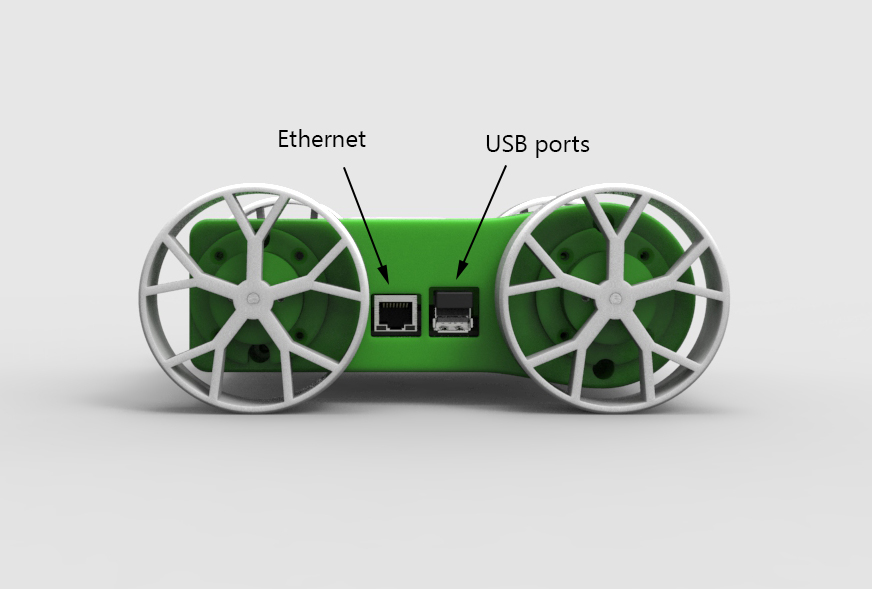
\includegraphics[width=350px]{render/pibotstarboard.jpg}
\centering
\end{figure}

\begin{figure}[!htbp]
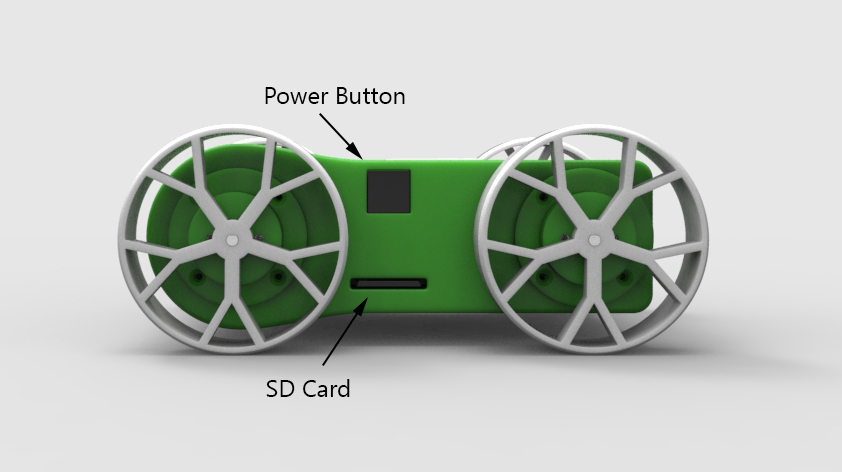
\includegraphics[width=350px]{render/pibotport.jpg}
\centering
\end{figure}

\begin{figure}[!htbp]
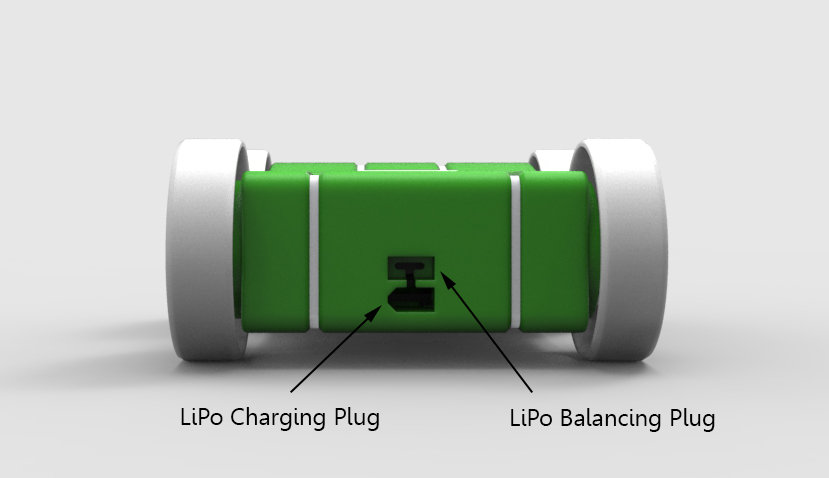
\includegraphics[width=350px]{render/pibotback.jpg}
\centering
\end{figure}

\pagebreak
\chapter{Bill of Materials and Required Tools}
\section{Parts and Tools}

The following tables provide a list of the parts and tools required to build the rover. The parts are currently sourced from many suppliers resulting in many orders and higher shipping costs. 
After additional development is complete, we may offer a single source supply for all components necessary to build the rover. Table \ref{table:BOM} lists the major components of the rover. Table \ref{table:opBOM}. The basic tools required are found in Table \ref{table:tools}. A list of screws required for assembly is found in Table \ref{table:screws}. The wiring components are in Table \ref{table:wires}. The instructions for the assembly of the circuit board and a list of the required components are given in a later section.

\begin{table}[!h]
\begin{tabular}{p{4cm} | p{3.5cm} | c | c | c}
part & supplier &  quantity &   total cost & image\\
\hline
12V 100rpm 25mm gearmotors & ebay, aliexpress, amazon&  4  & \$40 & 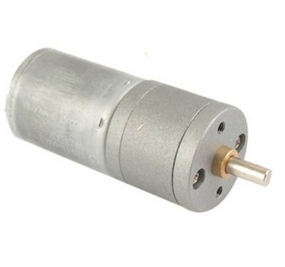
\includegraphics[width=80px]{picture/motor.png}\\
Raspberry Pi B, B+, 2 & adafruit, element14 & 1 & \$40-\$60 & 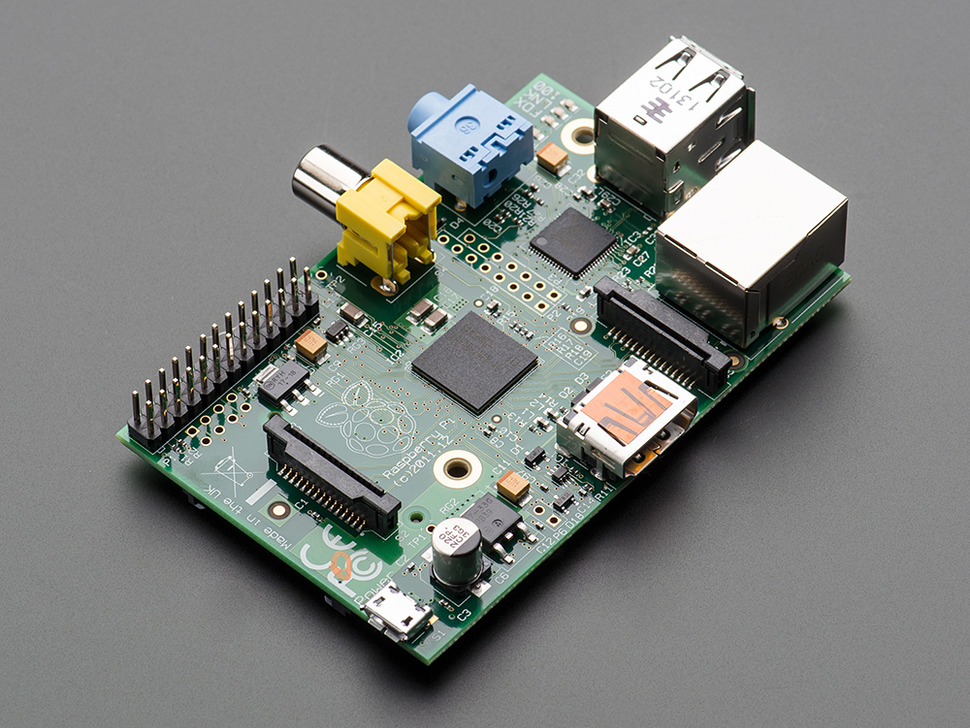
\includegraphics[width=80px]{picture/pi.jpg}\\
Raspberry Pi Wifi USB Adapter & adafruit, element14 & 1 & \$12 & 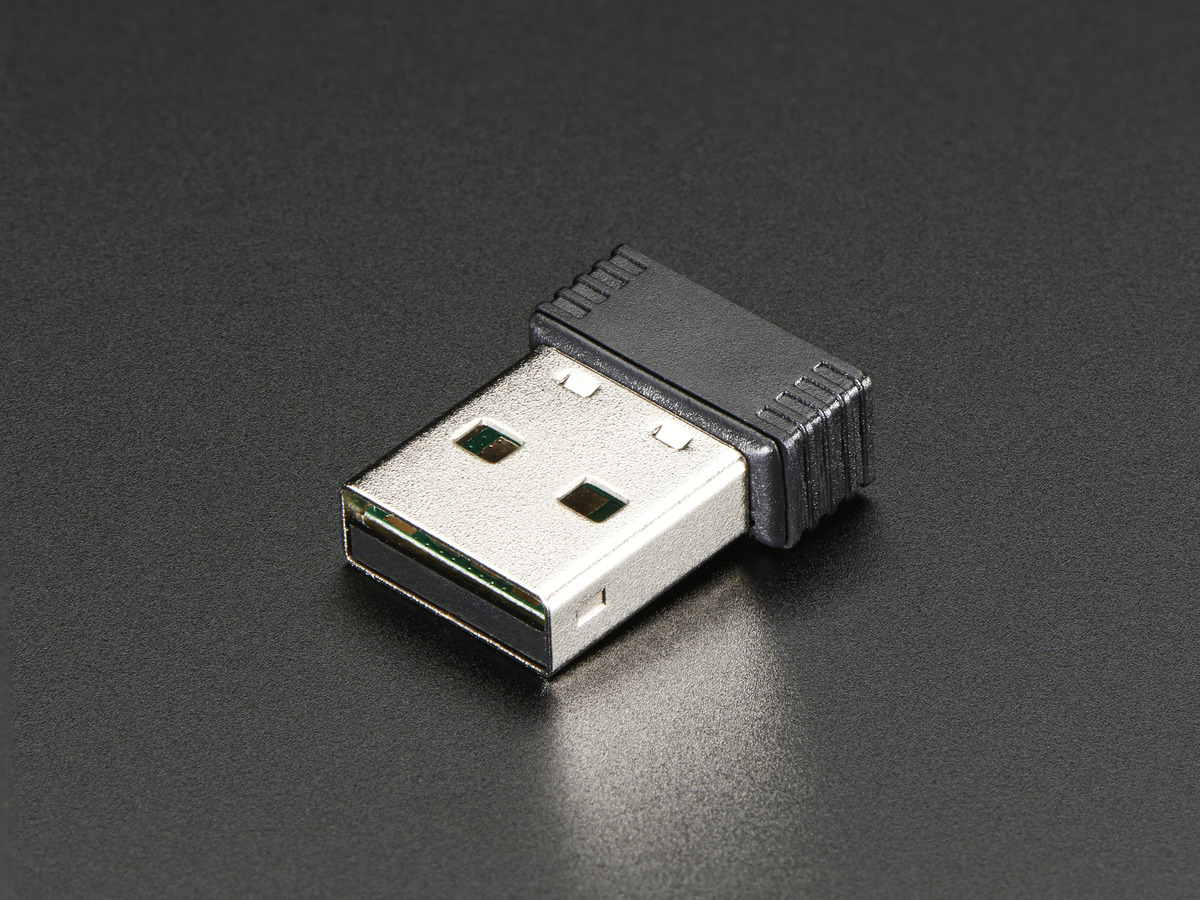
\includegraphics[width=80px]{picture/piwifi.jpg}\\
Raspberry Pi Camera Board, NoIR & adafruit, element14 & 1 & \$30 &  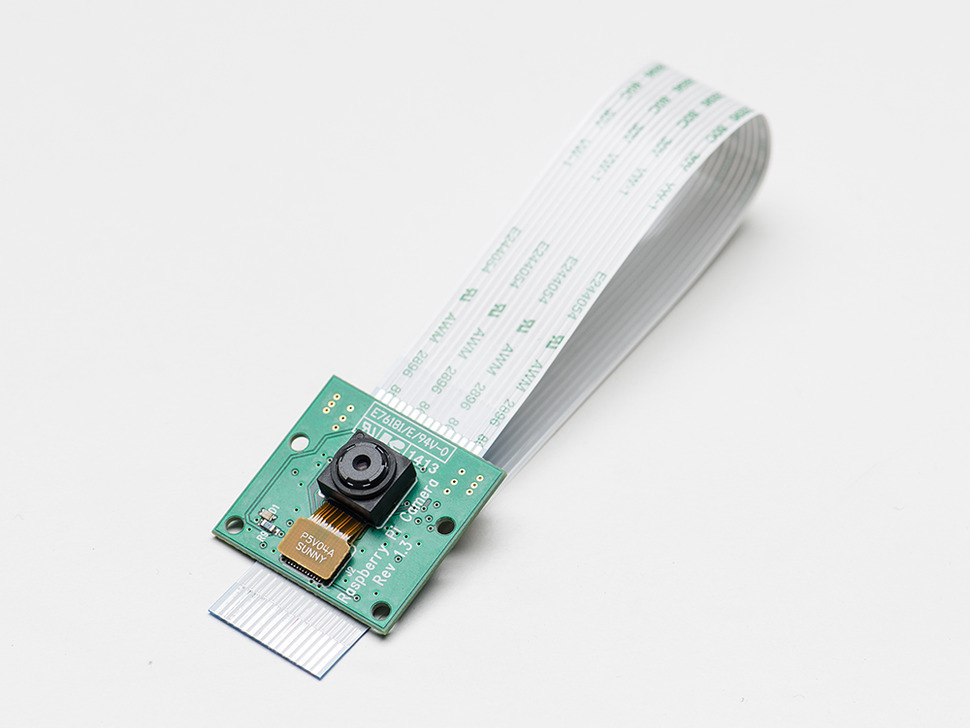
\includegraphics[width=80px]{picture/picam.jpg}\\
SD card & & 1 & \$15 & NA\\
Turnigy 2200mAh 3S 20C LiPo Pack & HobbyKing & 1 & \$10 &  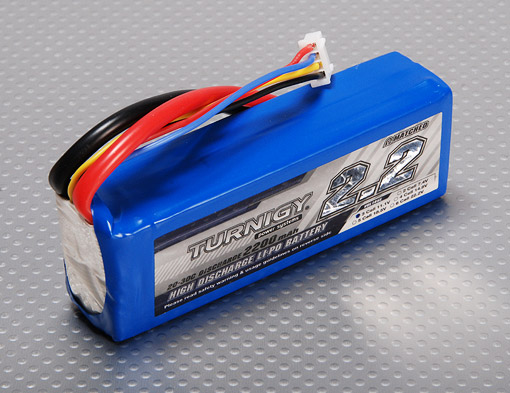
\includegraphics[width=80px]{picture/lipo.jpg}\\
Raspberry Robot Electronics Board & None & 1 & N/A &  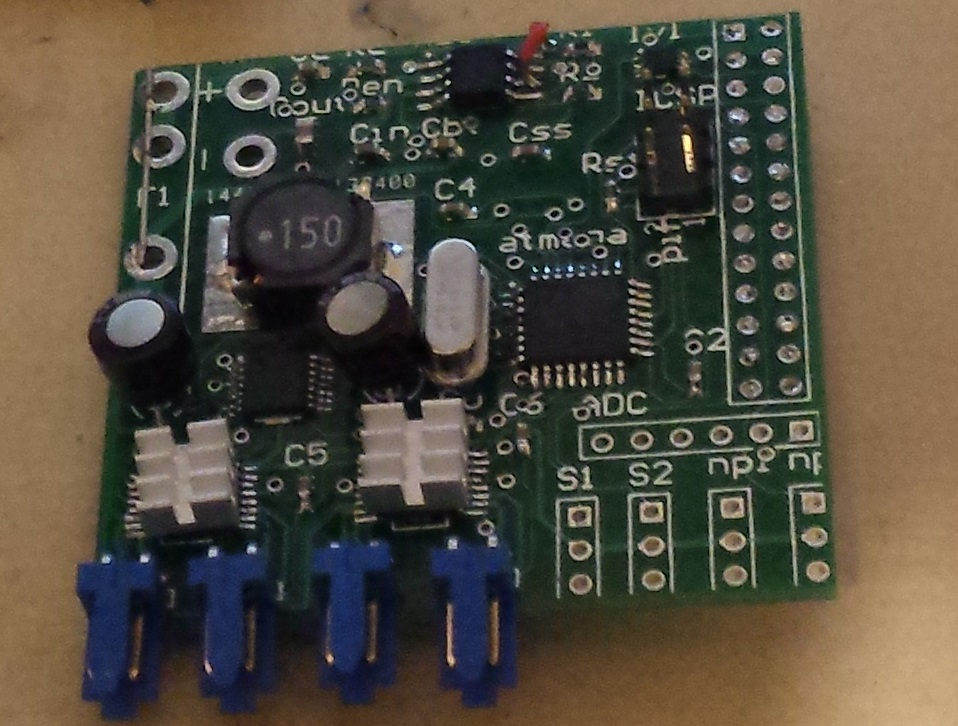
\includegraphics[width=80px]{picture/piboard.jpg}\\
Lithium Polymer B3AC Battery Charger & HobbyKing & 1 & \$8 & 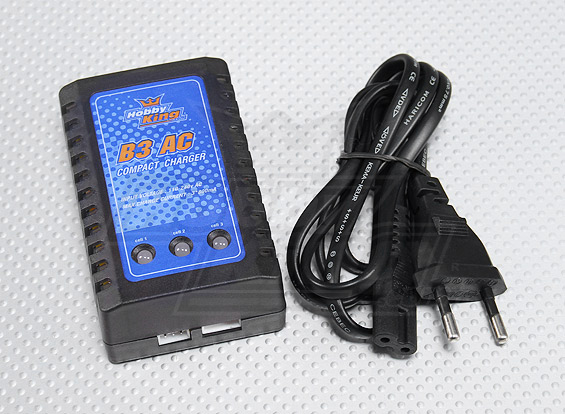
\includegraphics[width=80px]{picture/charger.jpg}\\
Wiring and connectors & NA & 1 & \$15 & NA \\
Screws and bolts & NA &1 & \$10 & NA \\
3D printed parts & NA & 12 & \$30 filament & NA \\
\end{tabular}
\caption{Major Components Bill of Materials}
\label{table:BOM}
\end{table}

\begin{table}[!h]
\begin{tabular}{p{4cm} | p{3.5cm} | c | c | c}
part & supplier &  quantity &   total cost & image\\
\hline
Logitech F710 Gamepad & Bestbuy, computer stores & 1  & \$45 & 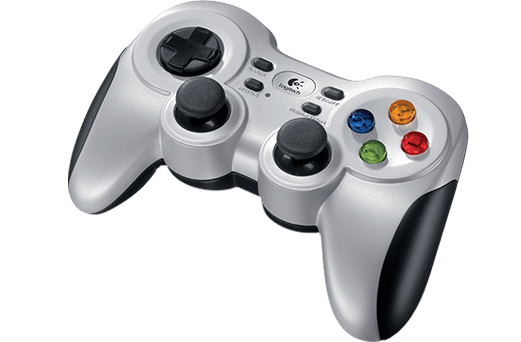
\includegraphics[width=80px]{picture/f710.png}\\
\end{tabular}
\caption{Optional Equipment}
\label{table:opBOM}
\end{table}

\begin{table}[!h]
\begin{tabular}{c | c}
\hline
recommended tools & \\
\hline
Hex key set (metric) 1.5,2,2.5,3mm sizes & 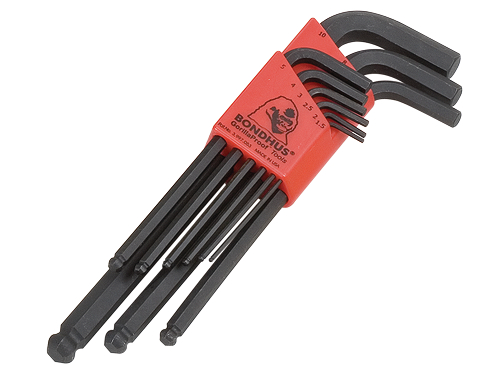
\includegraphics[width=80px]{picture/hexkey.jpg}\\
Soldering Iron with medium and fine tips & 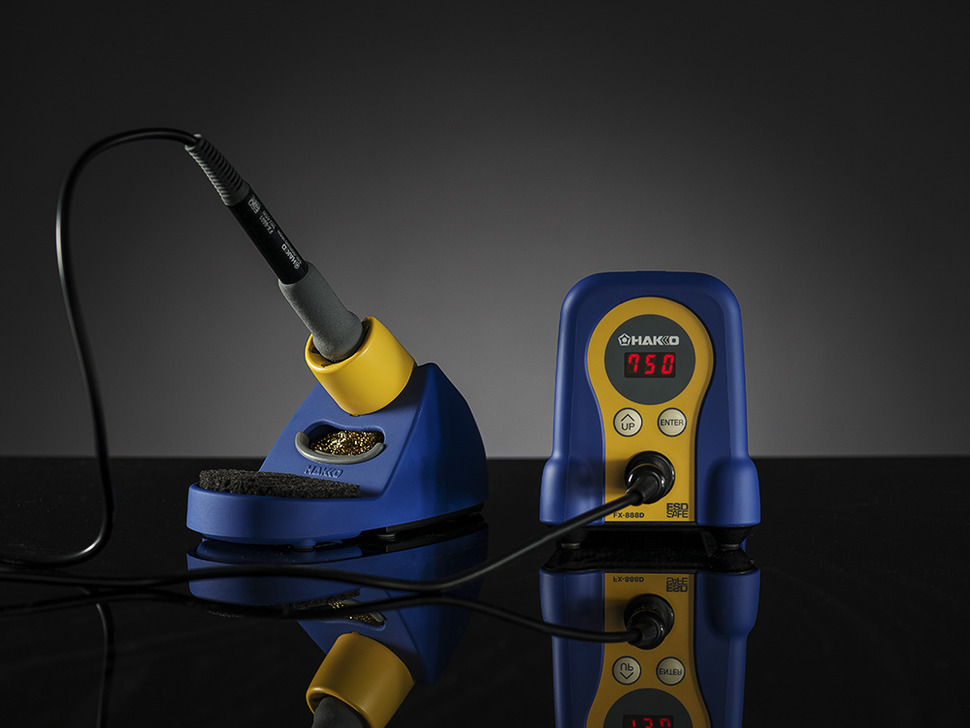
\includegraphics[width=80px]{picture/solderingiron.jpg}\\
Hobby Knife & 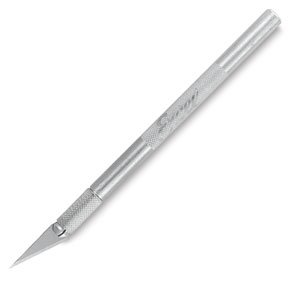
\includegraphics[width=80px]{picture/knife.jpg}\\
Wire strippers & 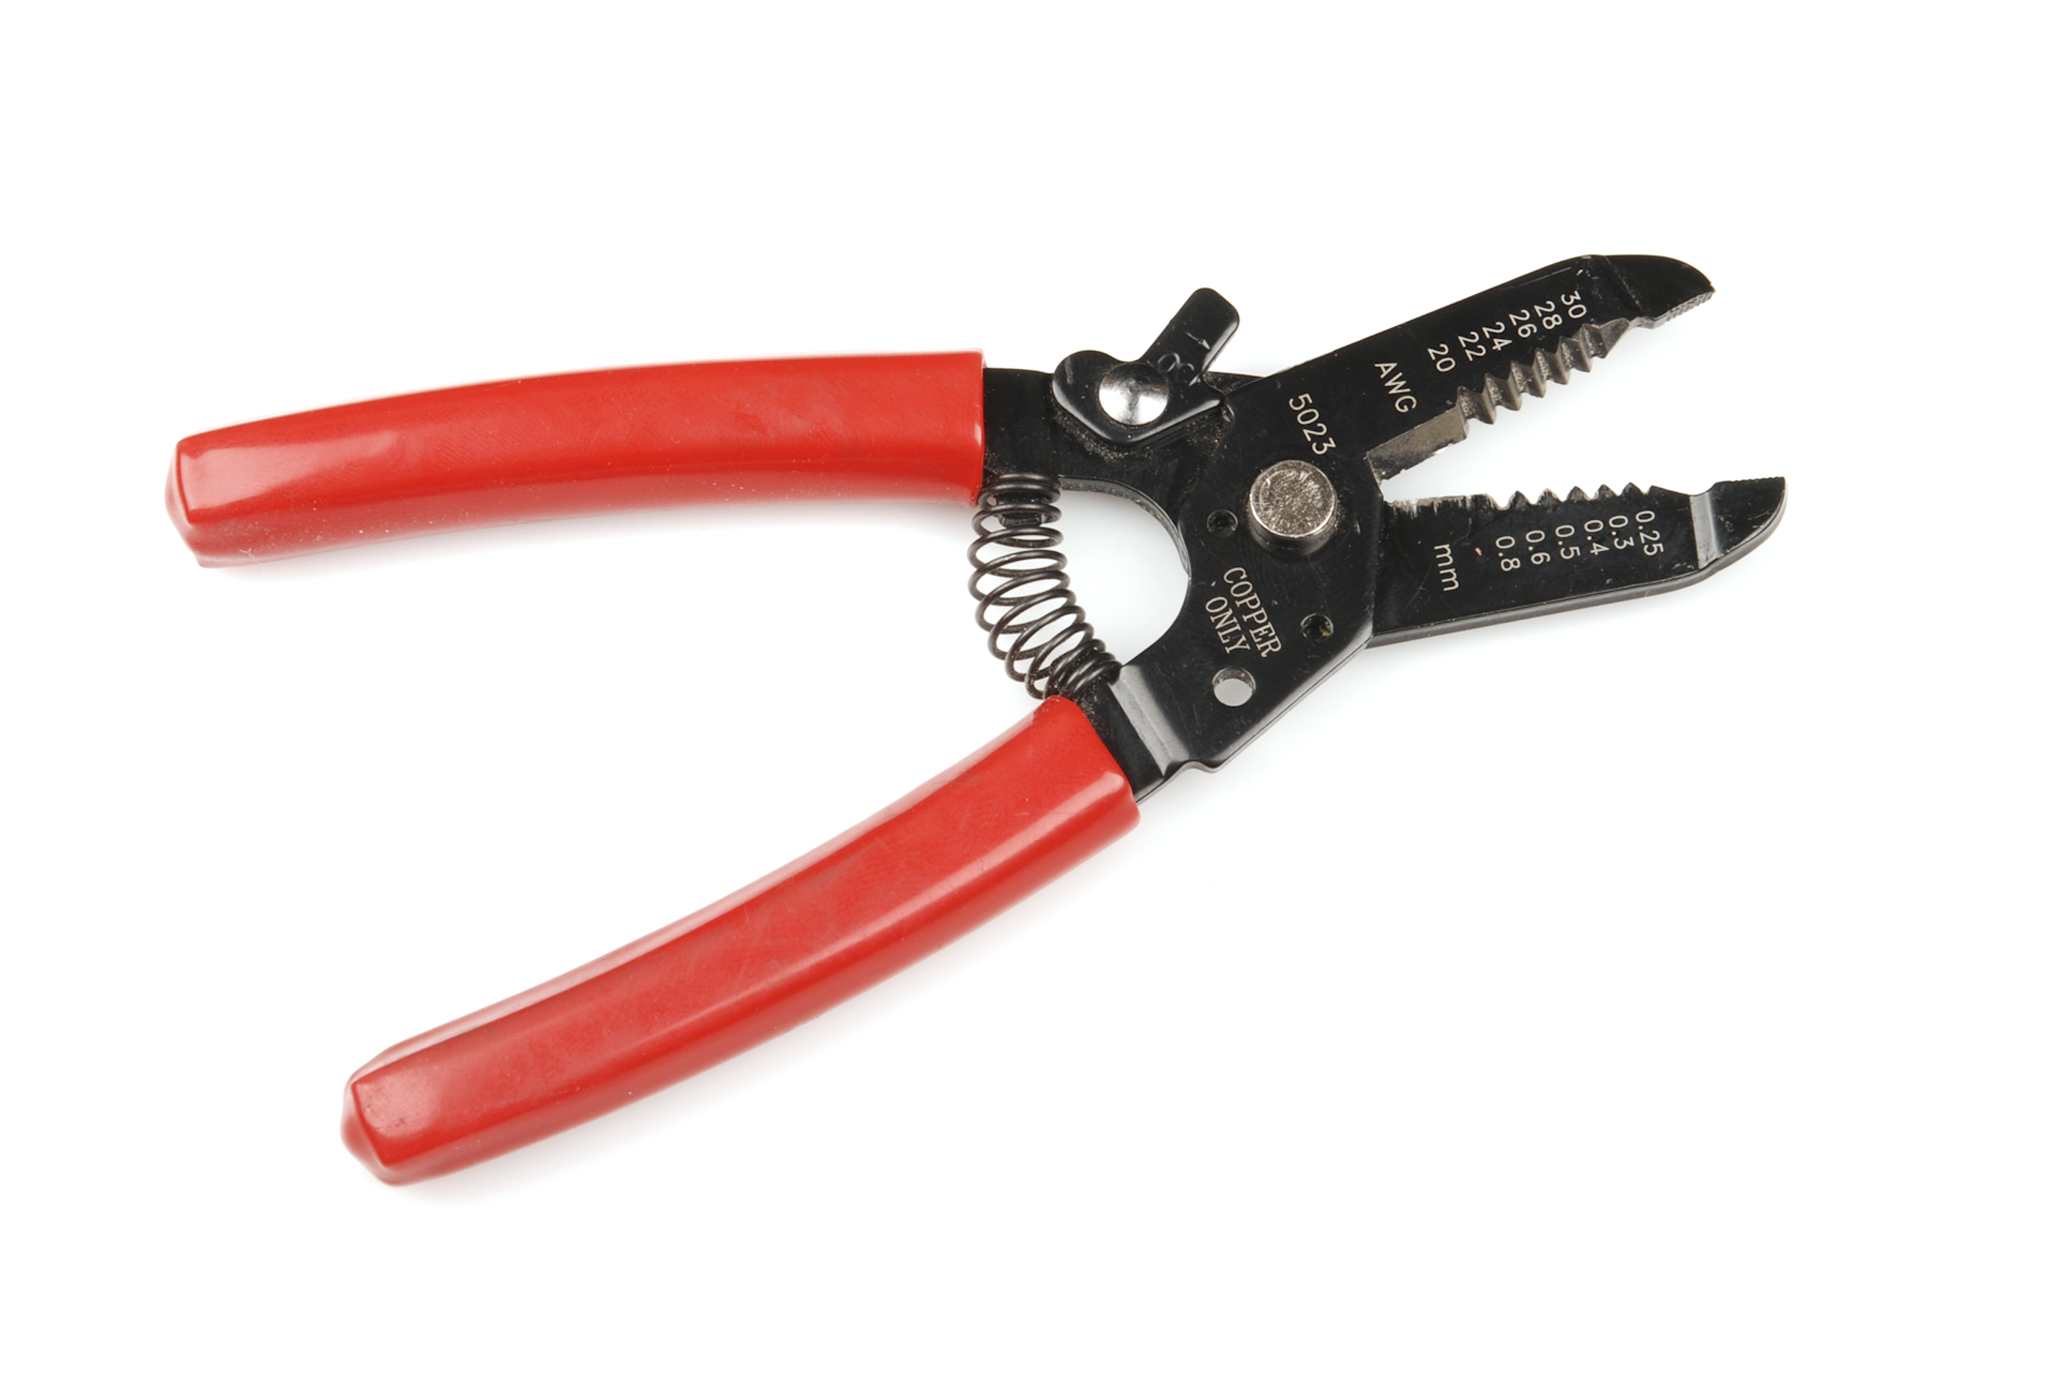
\includegraphics[width=80px]{picture/wirestripper.jpg}\\
AVR ISP mkii & 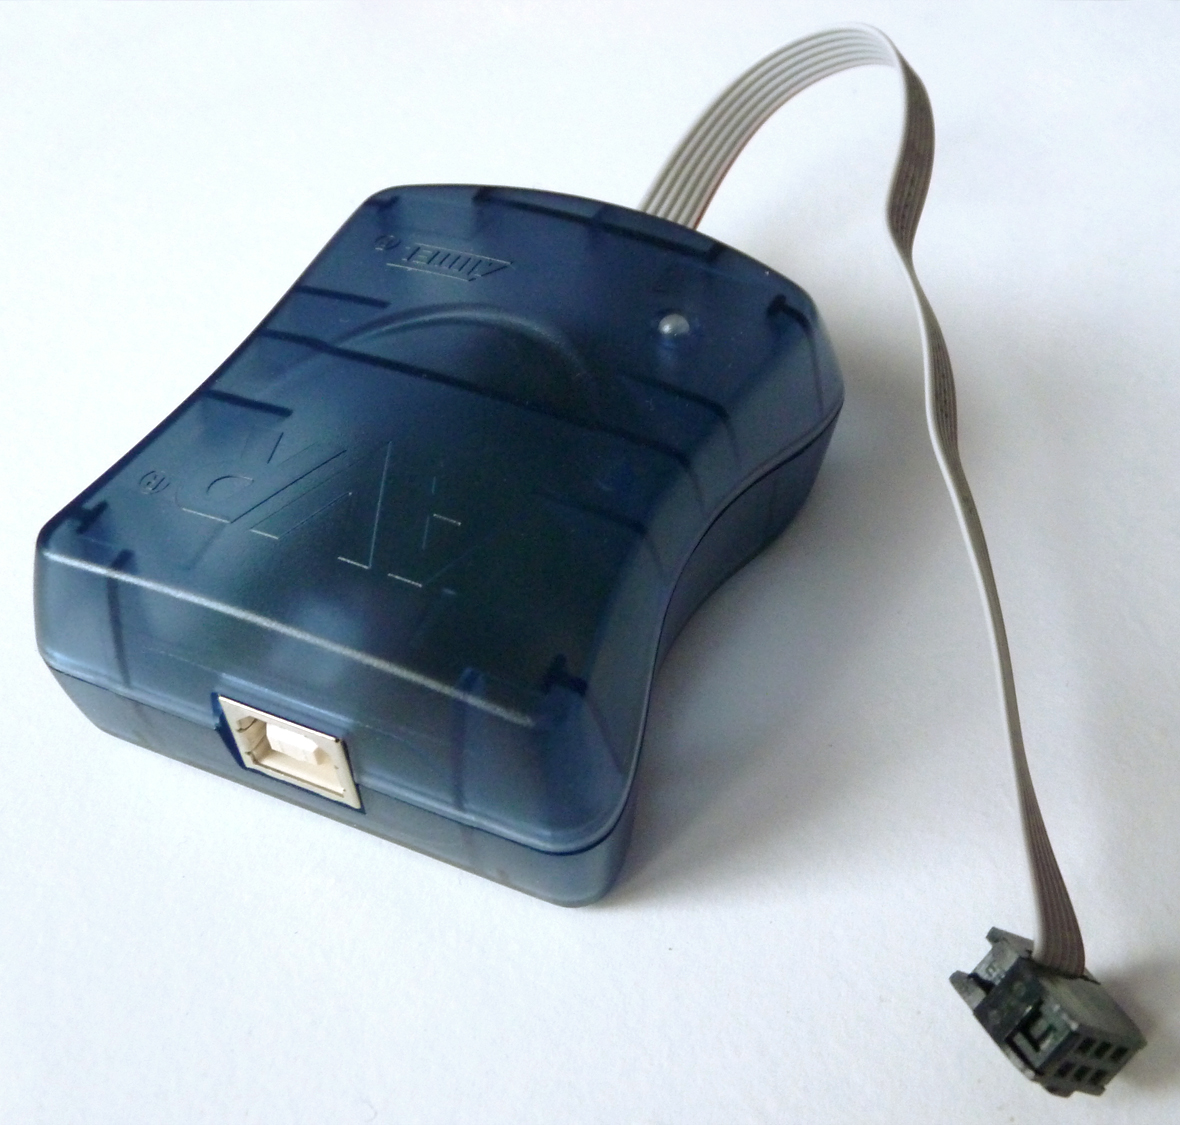
\includegraphics[width=80px]{picture/avrisp.jpg}\\
\hline
optional tools & \\
\hline
M3, M4 drill taps  & 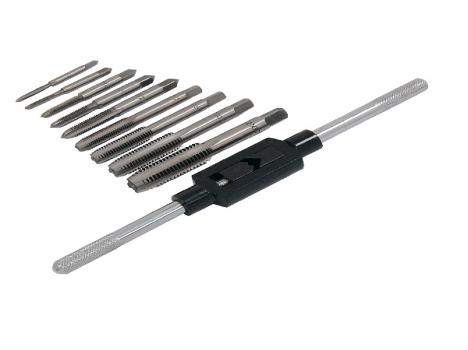
\includegraphics[width=80px]{picture/taps.jpg}\\
Hobby Tweezers & 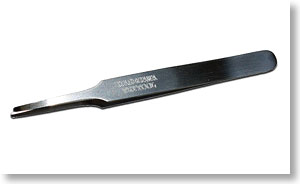
\includegraphics[width=80px]{picture/tweezer.jpg}
\end{tabular}
\caption{Recommended Tools}
\label{table:tools}
\end{table}


\begin{table}[!h]
\begin{tabular}{p{5cm} | c | c | c }
part & Spaenaur part number & quantity & image \\
\hline
Hex Socket Cap Screw M4 x 0.7mm x 25mm Full Thread & 367-022 & 4 & 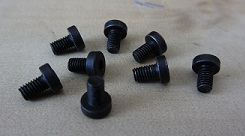
\includegraphics[width=80px]{hw/M3X06LHC.jpg}\\
Hex Socket Low Head Cap Screw M3 x 0.5mm x 5mm	& 366-1071 & 12 & 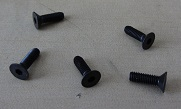
\includegraphics[width=80px]{hw/M3X10FC.jpg}\\
Hex Socket Flat Head Cap Screw M3 x 0.5mm x 10mm & 366-566 & 18 & \\
Hex Socket Cap Screw M3 x 0.5mm x 10mm & 367-B04-1P	& 5 & \\
Hex Socket Cap Screw M2 x 0.4mm x 6mm	& 366-663 & 4 & \\
\end{tabular}
\caption{Bill of Nuts and Bolts}
\label{table:screws}
\end{table}

\begin{table}[!h]
\begin{tabular}{p{5cm} | c | c | c | c}
part & supplier & part number & quantity & image \\
\hline
Hook up wire 20-22AWG & various, adafruit & adafruit 1311 & various colors & 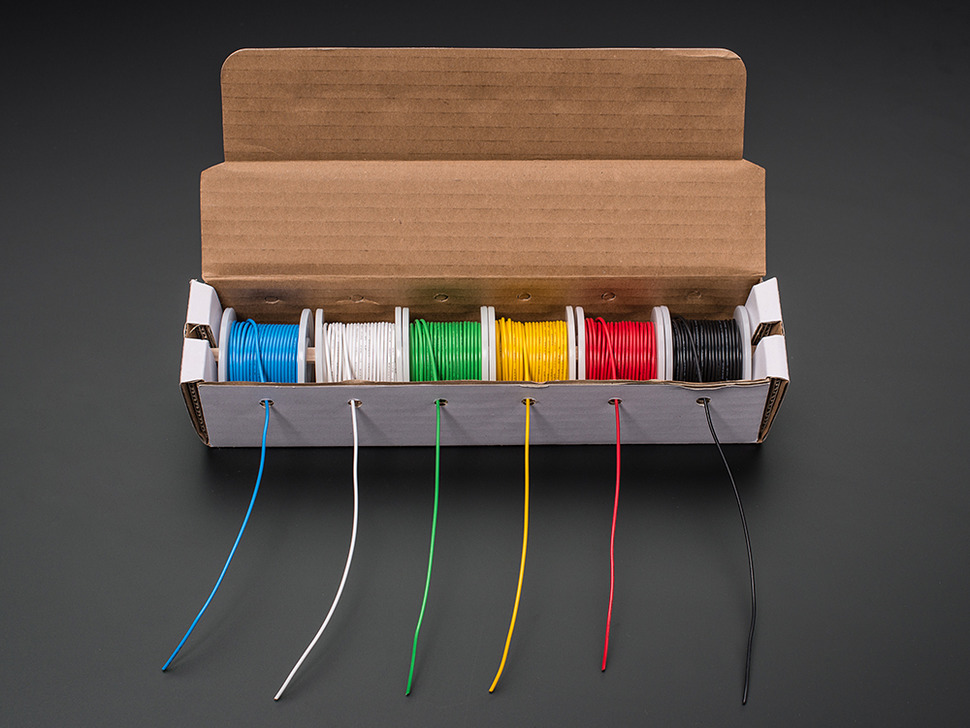
\includegraphics[width=80px]{picture/wires.jpg}\\
Female JST-XH <-> Male Polyquest 3S 10cm (5pcs/bag) & HobbyKing & 101b-103a-3s & 1 & 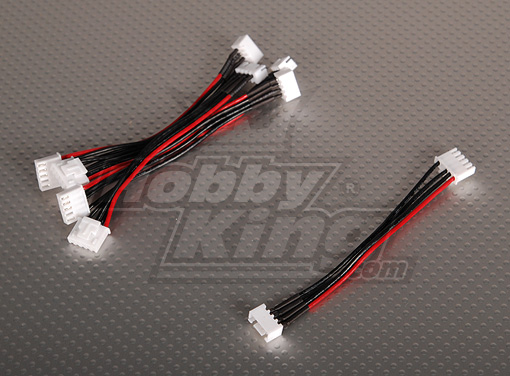
\includegraphics[width=80px]{picture/jstext.jpg}\\
Female JST battery pigtail 12cm length & HobbyKing & AM-9017A & 2 & 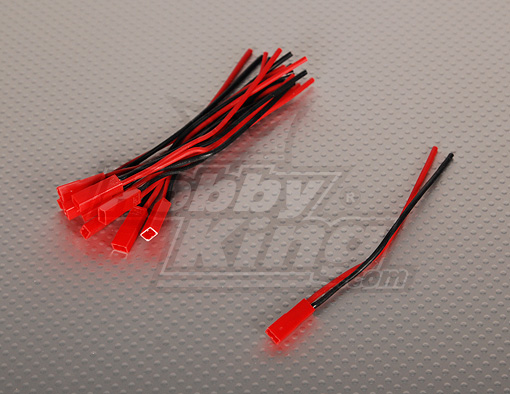
\includegraphics[width=80px]{picture/fjst.jpg}\\
Male JST battery pigtail 10cm length & HobbyKing & AM-9017B & 2 & 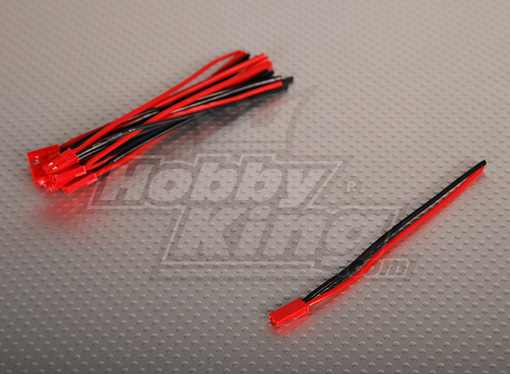
\includegraphics[width=80px]{picture/mjst.jpg}\\
Power Switch SPST & SW627-ND & digikey & 1 & 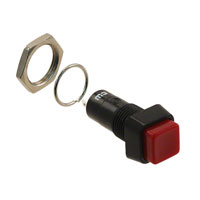
\includegraphics[width=80px]{picture/pwr.jpg}

\end{tabular}
\caption{Bill of Wires and Connectors}
\label{table:wires}
\end{table}


\section{3D printing}

The Raspberry Robot is made up of 8 unique 3D printed parts and a total of 12 3D printed pieces. The table: \ref{table:3Dprint} lists each part which is made with a 3D printer. The Raspberry Robot has been previously constructed with the printers listed and tested in Table: \ref{table:3Dprint}. Note that hex cap screws on this platform thread directly into 3D printed plastic. Holes have been sized appropriately to allow clearance for screws and appropriate diameters for threading. Appropriate hole sizing may vary printer to printer and should be checked on initial prints. Repeated screwing and unscrewing or forcing taps or screws may result in damage to 3D printed threaded holes.  

Some parts will require support material. All parts have been found to function well when printed at 20\% infill. 3D printing settings and parameter decisions will ultimately be left to the operator. 

\begin{table}
\begin{tabular}{p{5cm} | c | c | c}
part & quantity & image & support material required\\
\hline
Side Left V01 & 1 & 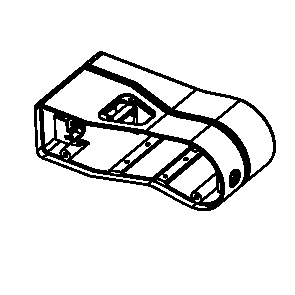
\includegraphics[width=70px]{diagram/Side_Left_V01.pdf} & yes\\
Side Right V01 & 1 & 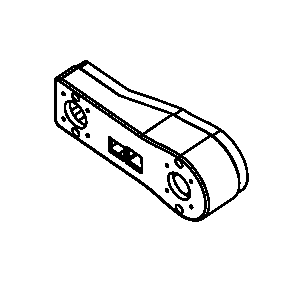
\includegraphics[width=70px]{diagram/Side_Right_V01.pdf} & not required\\
FR motor holder & 1 & 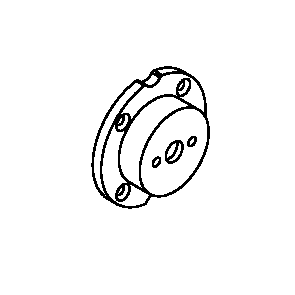
\includegraphics[width=70px]{diagram/FR_motor_holder.pdf} & yes\\
RR motor holder & 1 & 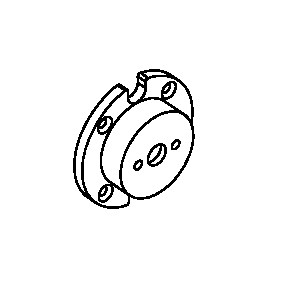
\includegraphics[width=70px]{diagram/RR_motor_holder.pdf} & yes\\
L motor holder & 2 & 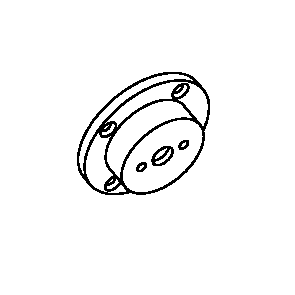
\includegraphics[width=70px]{diagram/L_motor_holder.pdf} & yes\\
PiTrayB & 1 & 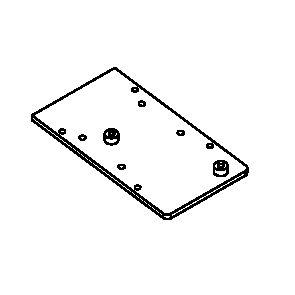
\includegraphics[width=70px]{diagram/PiTrayB.pdf} & not required\\
Top Plate & 1 & 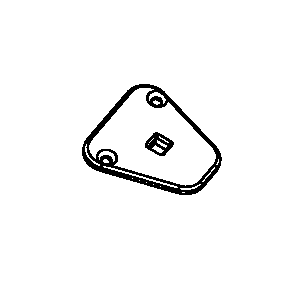
\includegraphics[width=70px]{diagram/Top_Plate.pdf} & not required\\
Wheel & 4 & 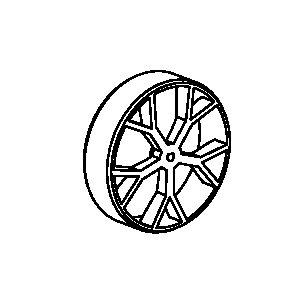
\includegraphics[width=70px]{diagram/Wheel.pdf} & not required
\end{tabular}
\caption{Bill of 3D printed components}
\label{table:3Dprint}
\end{table}

\begin{table}
\begin{tabular}{c | c | c | c}
printer & build volume & image& result quality\\
\hline
Makerbot Replicator 2 & 28.5 L X 15.3 W X 15.5 H cm & 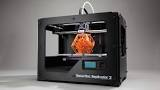
\includegraphics[width=70px]{picture/makerbotrep2.jpg} & excellent $\dfrac{10}{10}$\\
Tinkerines Ditto+ & 21.0 L X 18.5 W X 23.0 H cm  & 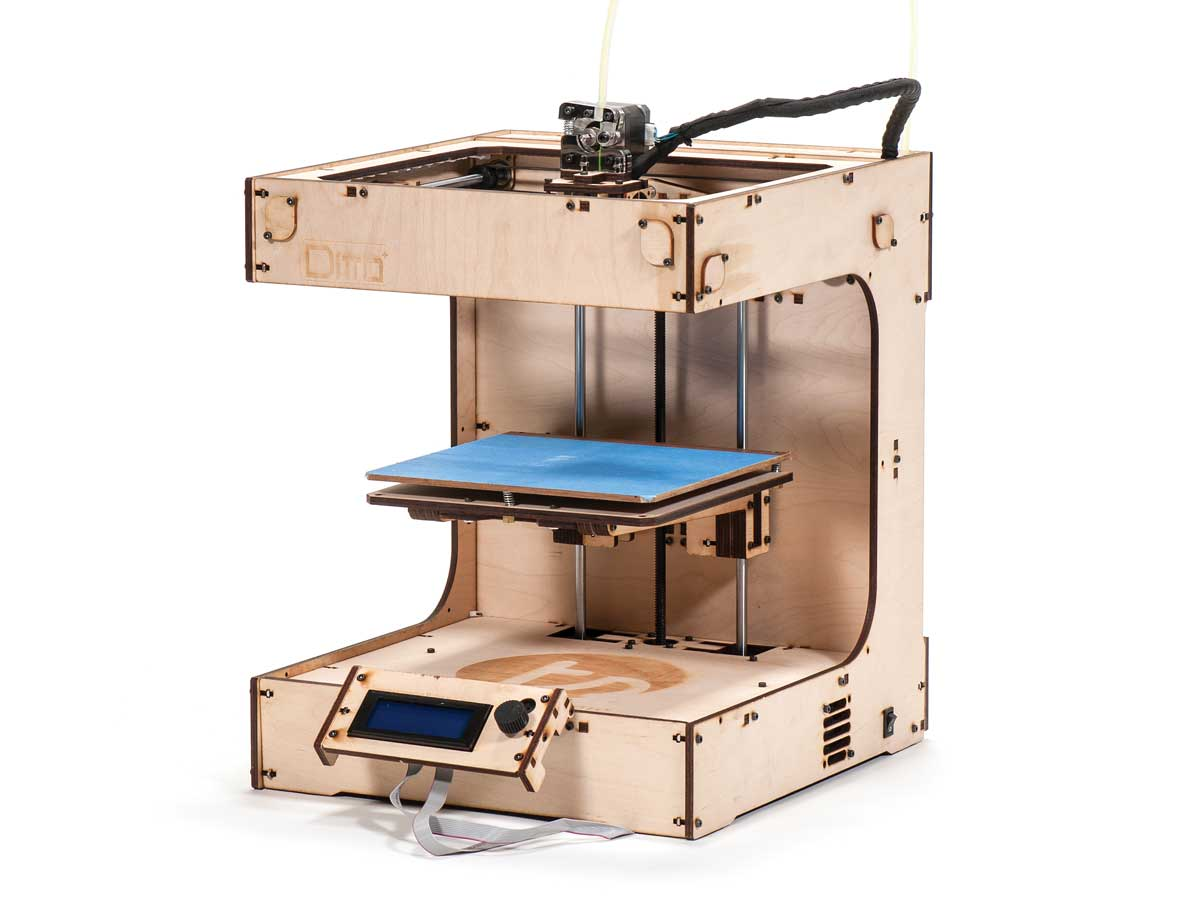
\includegraphics[width=70px]{picture/ditto.jpg} & very good $\dfrac{9}{10}$\\
 
\end{tabular}
\caption{3D printers used}
\label{table:3Dprint}
\end{table}




\chapter{Assembly}

The rover is easy enough to assemble but it isn't perfect, yet. Many components and wires are packed tightly into a small space. Screws may be difficult to access with hex keys. Once the vehicle has been assembled and is running properly, minimal disassembly and maintenance will be required. Once all the 3D printed components are available with support material removed assembly can begin.\\

\section{Electronics Assembly and Test}

\begin{enumerate}

\item Download the latest RaspberryRover SD card image from <MAKE A LINK>. Use a program such as Win32diskimager to mount it on to an 8GB SD card. Later when the image is booted, raspi-config can be used to expand the file system to fill the full 8GB of storage.
\item Plug the Raspberry Pi Camera and Wifi dongle into the Pi and insert the SD card for now. Connect the unit to an Ethernet port on your router. Use conventional wall power to power the unit.
	\begin{enumerate}
	\item  Using your router's user interface, locate the IP address of the Raspberry Pi. The initial hostname will appear as <color>pibot. This can be changed with raspi-config at a later time.
	\item SSH into the Raspberry Pi using the IP address from step 2.1. In windows this can be done with a free program such as \href{http://www.chiark.greenend.org.uk/~sgtatham/putty/download.html}{Putty}. Username and 			password as usual:\\
	username: pi\\
	password: raspberry\\
	\item Verify that ROS is running (robot upstart is used to start ROS and required nodes at boot up).\\
	\begin{verbatim}
		$rostopic list
	\end{verbatim}
	\item Verify the mjpg-streamer software has started and is streaming video from the camera. Point a web-browser to: Your bot's IP address:8080
	Configure the Wifi on the Pi to automatically connect to your network using wicd-curses.
	\begin{verbatim}
		$sudo wicd-curses
	\end{verbatim}
	\end{enumerate}

\item Attach the wire ends of a male JST pigtail connector to the Lithium Polymer battery.\\
	\begin{enumerate}
	\item Using a hobby knife, remove a small amount of shrink wrap from the battery ground (black) wire connection to the yellow XT-60 connector.
	\item Solder on the ground (black) wire to the JST connector
	\item repeat this process with the positive (red) connection on the yellow XT-60 connector
	\item Solder on the positive (red) lead from the JST connector\\
	\end{enumerate}
	\begin{center}\textbf{WARNING}\end{center}
	Take care not to short the battery terminals together while making this modification. Do not let the knife short the terminals while cutting!\\
	\begin{center}\textbf{WARNING}\end{center}
	Take care to check the polarity of the connection, red to red, black to black.
	\item Mount the MCU electronics board on top of the Raspberry-Pi. Ensure the GPIO connectors line up with the female header on the MCU board.
	\item Wire connectors to the electric motors
	\begin{enumerate}
		\item Cut 10cm lengths of two different colors of 20-22awg wire for each of the motors (4x color 1, 4x color 2)
		\item Solder one end of each wire to the motor terminals, ensure consistency of polarity. Check for the red dot on the motor by the terminal to find the positive connection.
		\item Build the 2pin blue connector (PART NUMBERS) on the other ends of the wires for each motor. Again, ensure consistency of polarity. Place positive on the right and side of the connector (connector slot faces upwards)	
	\end{enumerate}
	\item Attach the motors to the MCU board according to the diagram in FIGURE WHAT?
	\item Power up the system by connecting the Battery JST connector to the JST connector on the MCU board. The LED will illuminate in blue. The Pi should power on and boot as usual. 
	\item Verify the system has booted normally, SSH into the Pi and verify ROS and the camera have started.
	\item Verify the motors are operational by manually publishing their control ROStopic
	\begin{enumerate}
	
	\item Set all motors to full forward speed
	\begin{verbatim}
	$ rostopic pub /piBot_motors std_msgs/ColorRGBA 255 255 255 255
	\end{verbatim}
	\item Set all motors to full reverse speed
	\begin{verbatim}
	$ rostopic pub /piBot_motors std_msgs/ColorRGBA 0 0 0 0
	\end{verbatim}
	\item Set all motors to zero speed
	\begin{verbatim}
	$ rostopic pub /piBot_motors std_msgs/ColorRGBA 127 127 127 127
	\end{verbatim}
	Consider the location of each motor on the vehicle when noting the direction of travel of each
 motor.
 	\end{enumerate}
 	\item Verify the LED is responsive by publishing color topics. Set the light to red+green
 	\begin{verbatim}
 	$ rostopic pub /piBot_led std_msgs/ColorRGBA 180 120 0 0
 	\end{verbatim}
 	\item Verify the battery voltage is being monitored properly.
 	\begin{verbatim}
 	$ rostopic echo /piBot_bat
 	\end{verbatim}
\end{enumerate}
The electronics bring-up is complete

\section{Mechanical Assembly}

\begin{enumerate}
\item Attach the Pi-Tray to the left side of the chassis (PiTrayB to Side Left V01) using 2-4 Hex Socket Low Head Cap Screw M3 x 0.5mm x 5mm screws.\\
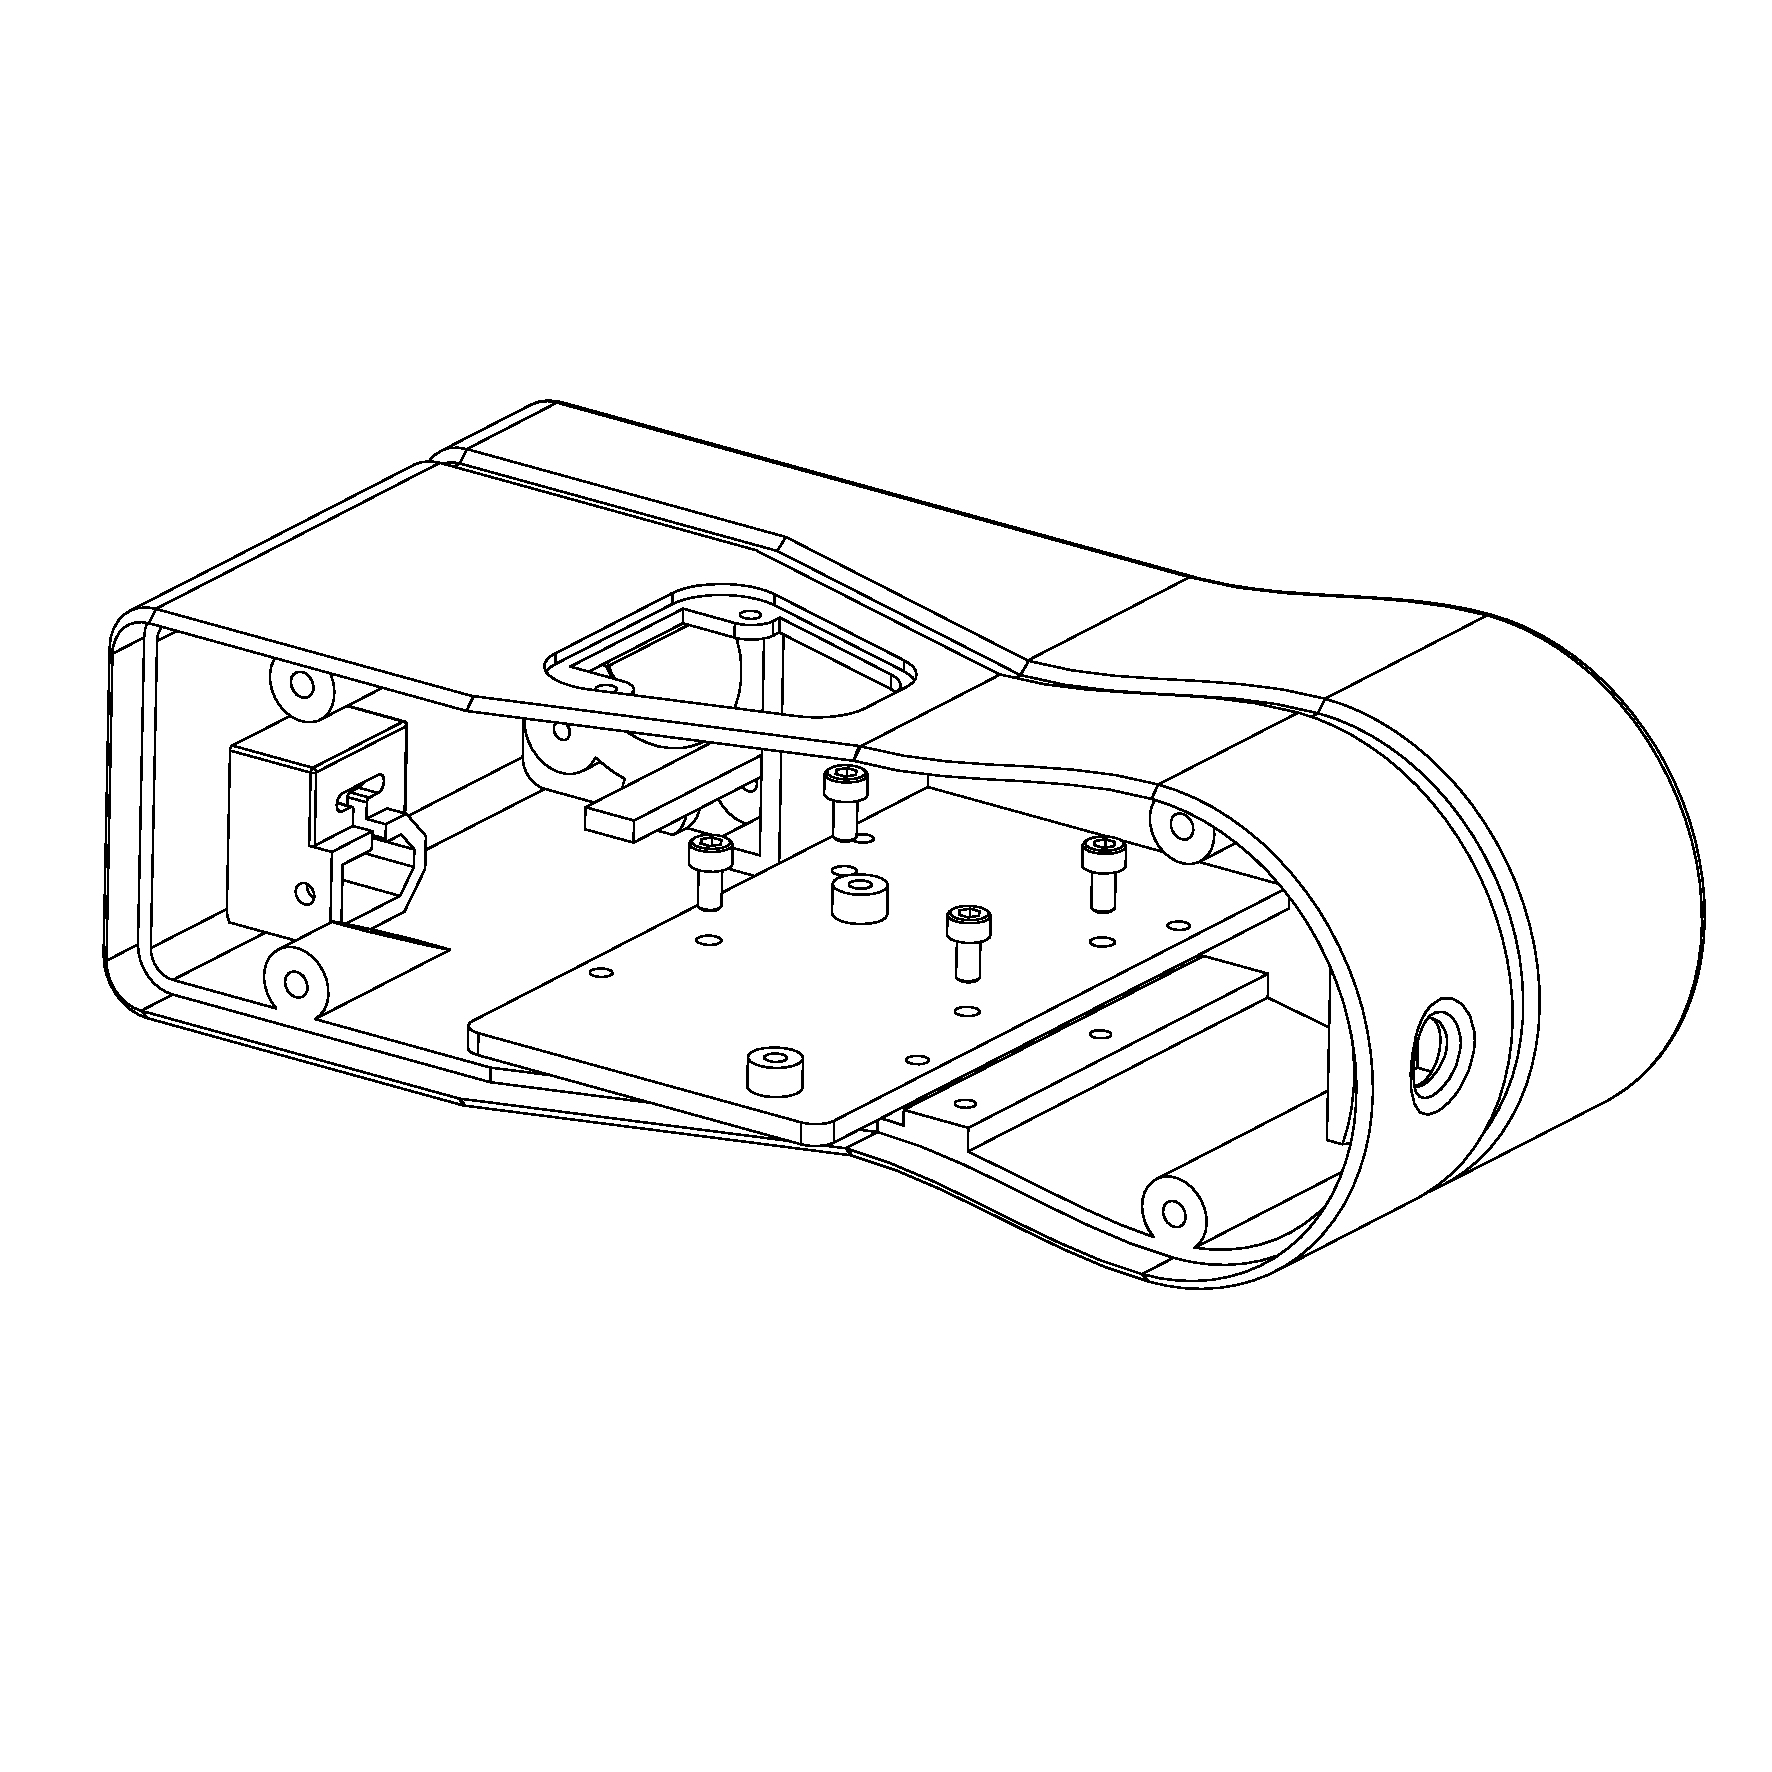
\includegraphics[width=400px]{assem/step1.PDF}
\item Mount the Pi-Camera to the inside of Side Left V01 using M2 Hex Cap Screws. Leave the ribbon cable attached to the camera board but not to the Pi during this process.
\item Install the Pi on the Pi mounting tray using M3 x 0.5 x 6mm Low Head Hex Cap screws
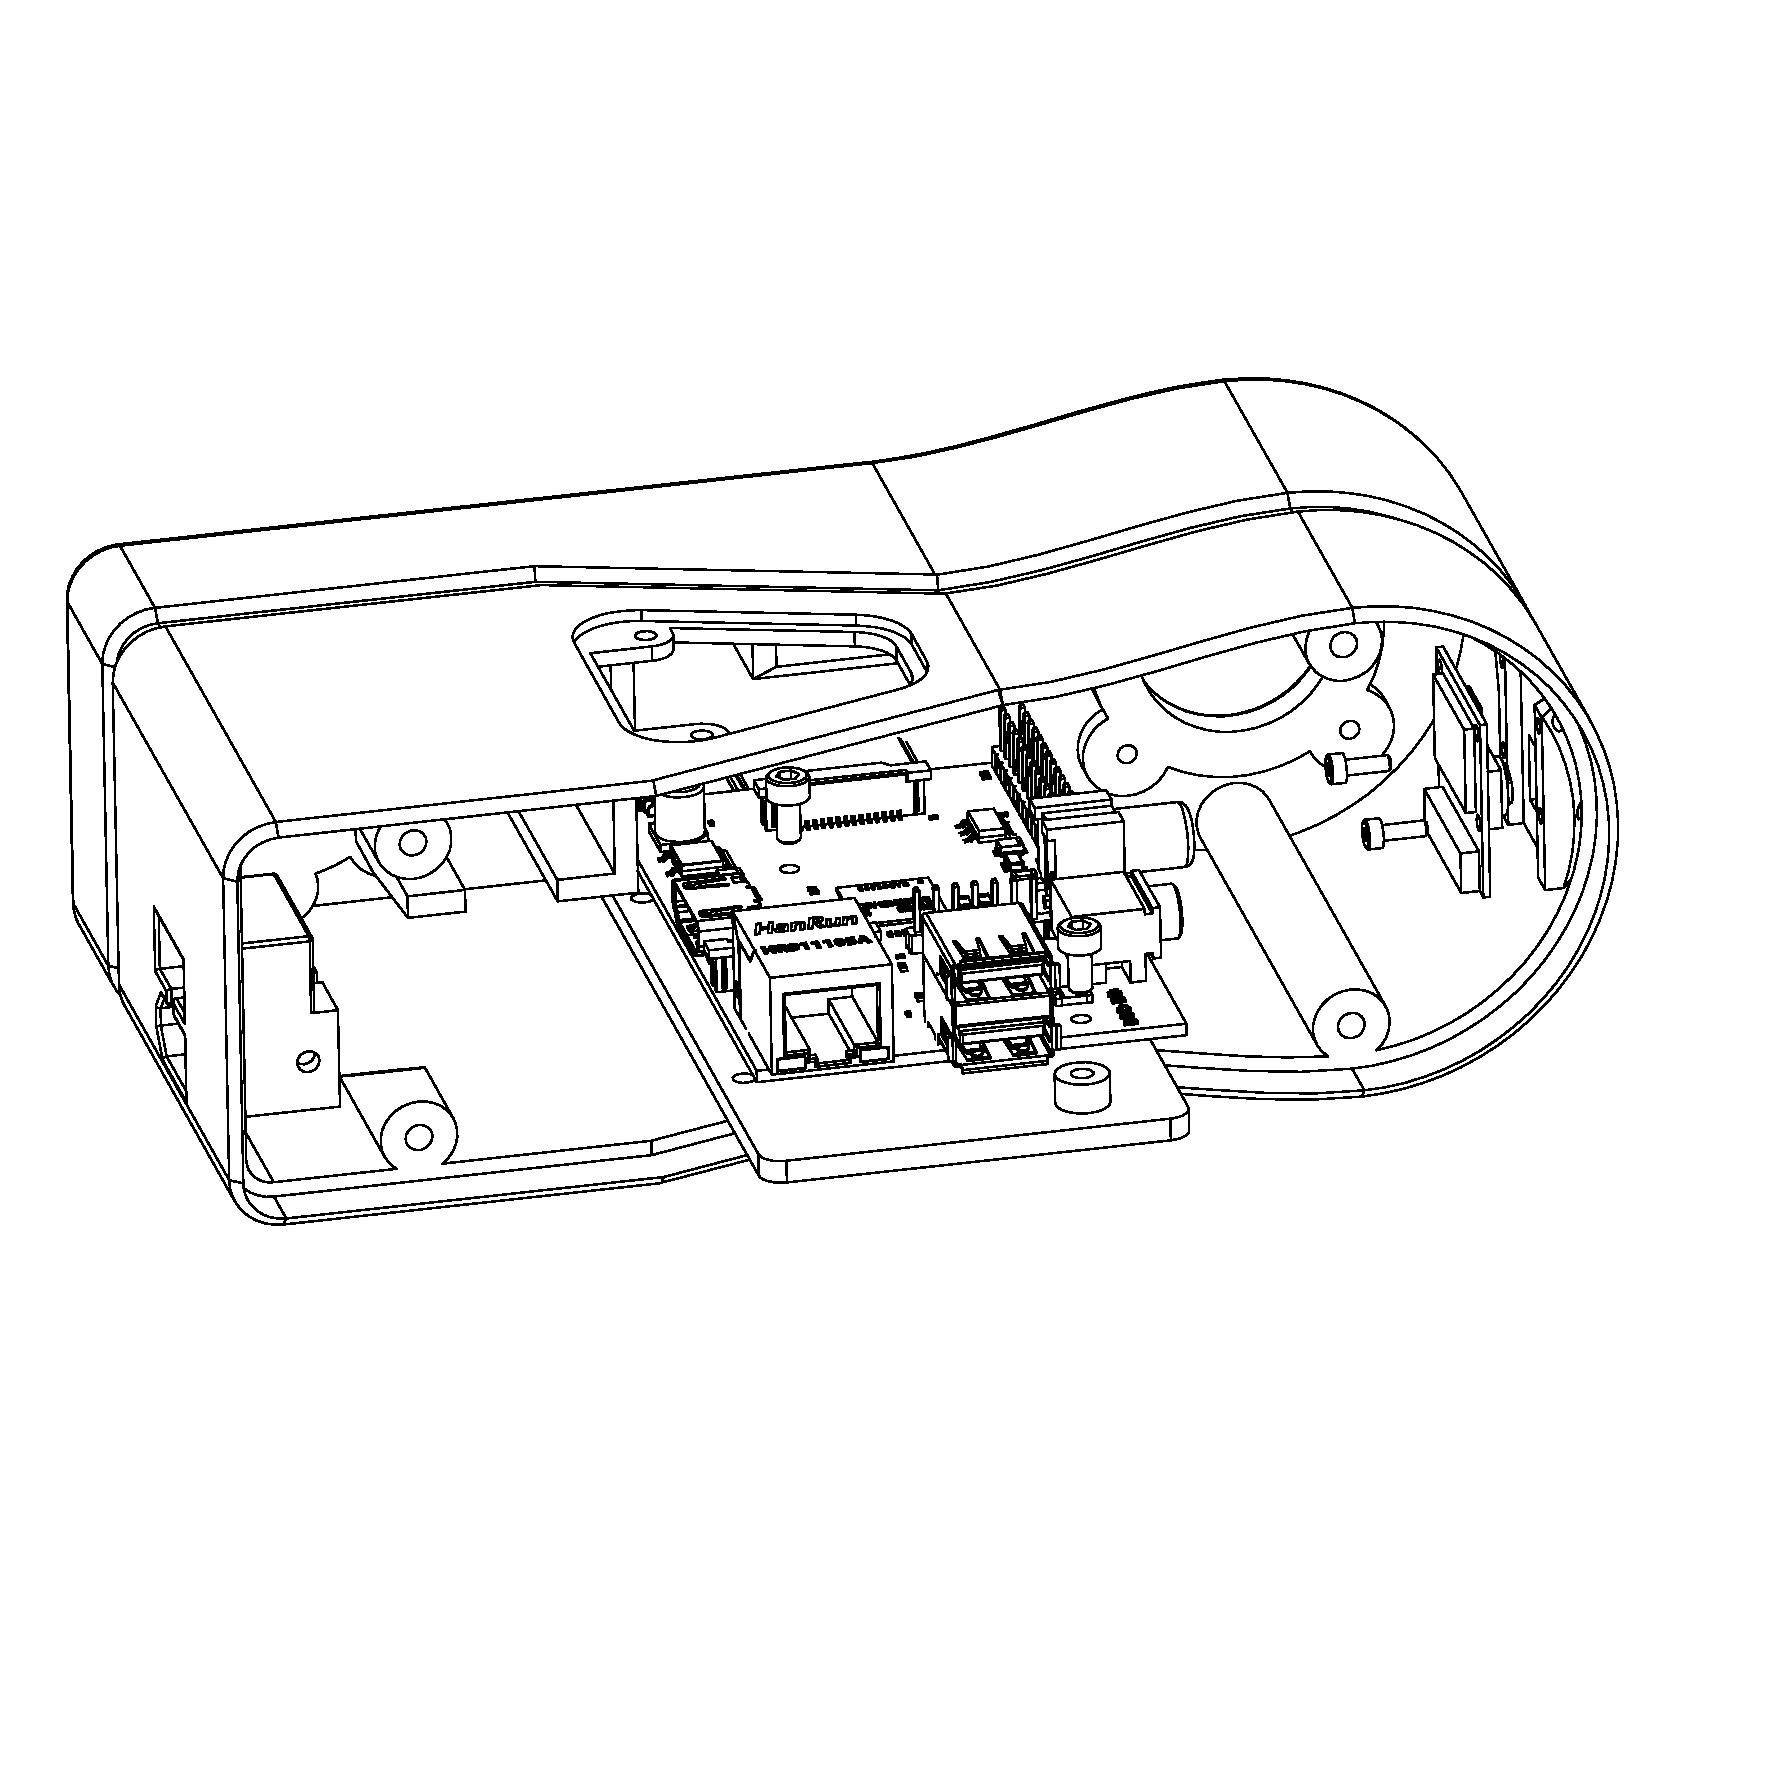
\includegraphics[width=400px]{assem/step2.PDF}[h]
\item  Attach the JST connectors to the power switch as shown in Figure <MAKE A FIGURE>. Positive power should run though the switch.
\item Install the switch into the slot in Side Left V01
\item Install the battery into Side Left V01. Before fully inserting the battery, run the balancing plug out the rear connection socket of the robot. This can be difficult, take care not to damage the wires. Next run the XT 60 out the corresponding rear connection socket. Run the JST back in the robot towards the Pi mounting tray. Fully insert the battery.
\begin{enumerate}
	\item Lock the XT-60 connector in place with the M3 x 0.5 x 6mm Low Head Hex Cap set-screw
\end{enumerate}
\item Connect the battery JST to the switch.
\item Connect the switched JST power to the MCU board. Test the functionality by turning it on. Ensure the electronics are not in contact with metal surface or other potential shorts during testing. Remove the MCU Board. 
\item Connect the Pi camera ribbon cable to the Pi.
\item Push the LED and wiring through the hole in Side Left V01. Attach the LED to the Top Plate. Screw the Top plate down to Side Left V01 using M3 x 0.5 x 10mm Flat Head Hex Cap screws.\\
\item Install the motors in each of the motor holders using M3 x 0.5 x 6mm Low Head Hex Cap screws.
\item Push the wheels on to the motor shafts. This may require a tap from a hammer. Use M3 x 0.5 x 10mm set screws in the wheels if required.
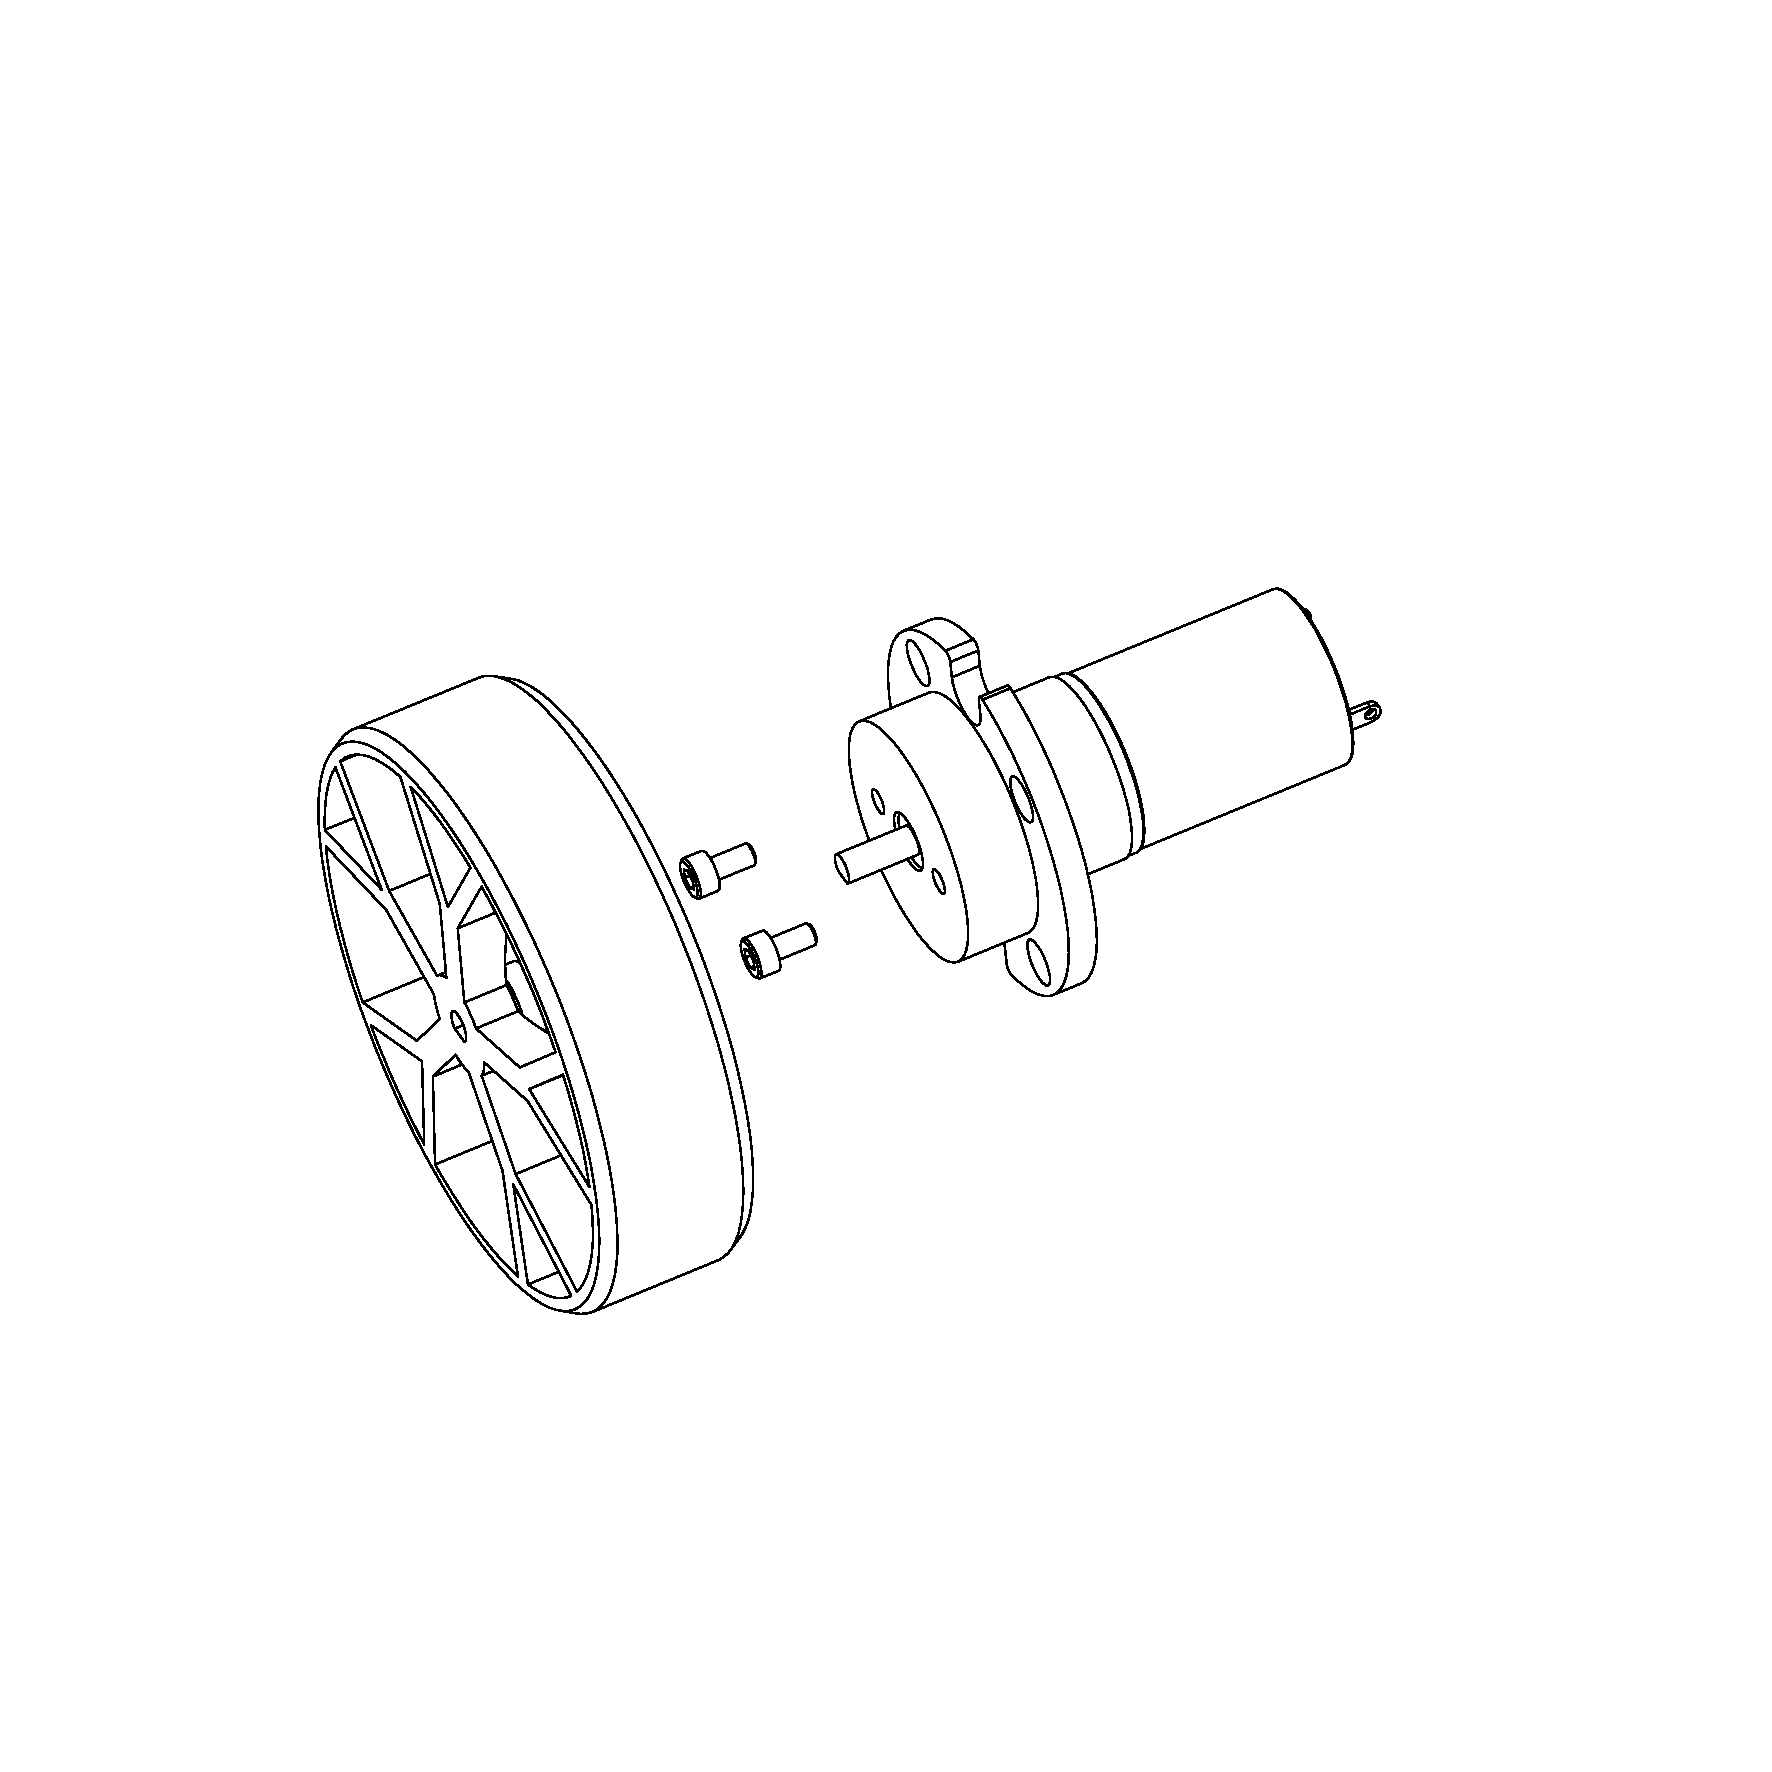
\includegraphics[width=400px]{assem/step3.PDF}[h]
\item Install the motor holder assemblies into the vehicle chassis sides (Side Left V01, Side Right V01)
\item Connect the motor wires to the MCU board in proper order shown in Figure XXX. You may wish to verify proper operation of the electronics one more time at this points
\item Push the two sides of the vehicle together while taking care not to tangle or stress wiring. This may take patience. 
\item Use four M4 x 0.7 x 25mm bolts to attach the chassis sides together.

\end{enumerate}

Mechanical assembly is complete.

\chapter{Operation}




\begin{appendices}
\chapter{Special Thanks}
Person 1\\
Person 2
\end{appendices}





\end{document}